\section{Replacement Strategy}
\label{ch:replacement_strategy}

This chapter describes the algorithm of restricted tournament replacement (RTR). Then, we focus on replacement strategy and discuss the effect of RTR on permutation problem. Thus, we define three various types of distance functions for restricted tournament replacement : edge distance, node distance, and order distance.


\subsection{Restricted Tournament Replacement}
The restricted tournament replacement (RTR) is a famous niching technique in the field of EDAs. RTR is also known as restricted tournament selection (RTS) which is first proposed in \citep{harik1995rts}. RTR is able to keep diversity. We present the process of RTR in algorithm \ref{alg:RTR_algorithm},where the Distance function is usually the Hamming distance function in binary problem. However, Hamming distance function is not suitable for permutation problem. Thus, we define new distance function for permutation problem according to characteristics of permutation problem.


\begin{algorithm}[htbp]
    \SetKwRepeat{doWhile}{do}{while}
    \KwIn{The original population $X=\lbrace x_1, x_2, ..., x_{n-1}\rbrace$\;
    The offspring population $Y$\;
    The window size $w$\; }
    \KwOut{The population $X$ of the next generation;}
    \For{ $y\in Y$ }
    {
        Choose a random subset $S =\lbrace s_0, s_2, ..., s_{w-1}\rbrace (0\leq s_i <n)$\;
        Find the $x_{s_i}$ in $\mathop{\arg\min}_{{s_i} \in S} Distance(x_{s_i},y)$\;
        \If{$Fitness(y)>Fitness(x_{s_i})$}      {
        $x_{s_i} \leftarrow y$;
        }
        
    }
    return $X$\;
    \caption{RTR algorithm}
    \label{alg:RTR_algorithm}
\end{algorithm}

\subsection{Edge Distance}


An edge is connection between two nodes. Edge distance is calculated by different edge between two chromosomes. Let $D_{edge} (i,j)$ denote the edge distance between the two chromosomes $i$ and $j$, and \[ES_i=\lbrace\forall k(\pi_i(k\ mod\ L), \pi_i(k+1\ mod\ L)\rbrace.\] Thus, $D_{edge} (i,j)$ is calculated as follows:\[D_{edge} (i,j)=L-\vert ES_i\cap ES_j\vert.\]

\begin{figure}[htbp] 
        \centering
        \begin{subfigure}{0.4\textwidth}
            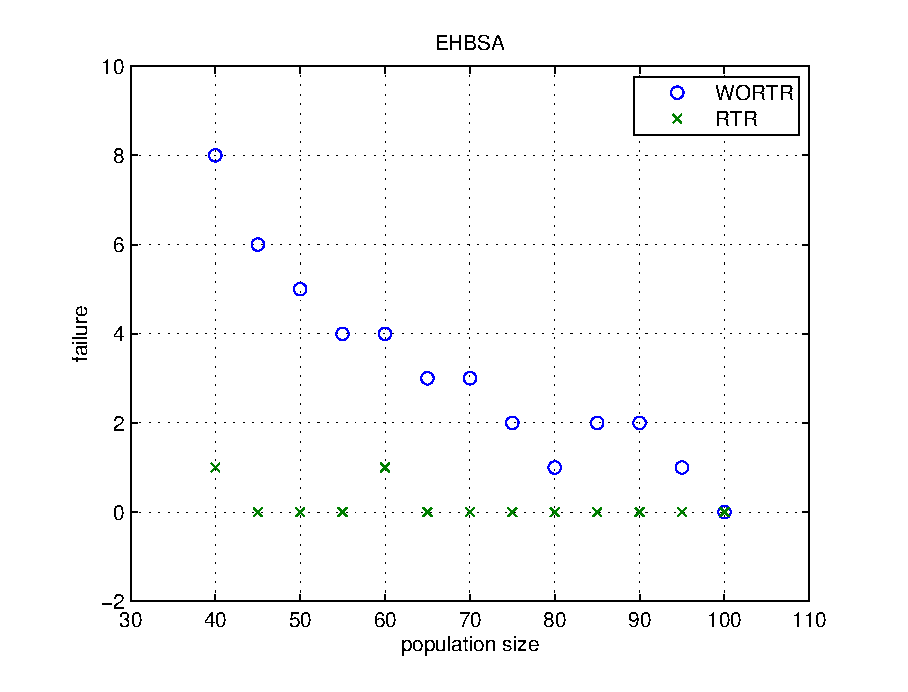
\includegraphics[width=\textwidth]{PF.eps}
            \caption{PopulationSize-Failure} 
        \end{subfigure}
        \begin{subfigure}{0.4\textwidth} 
            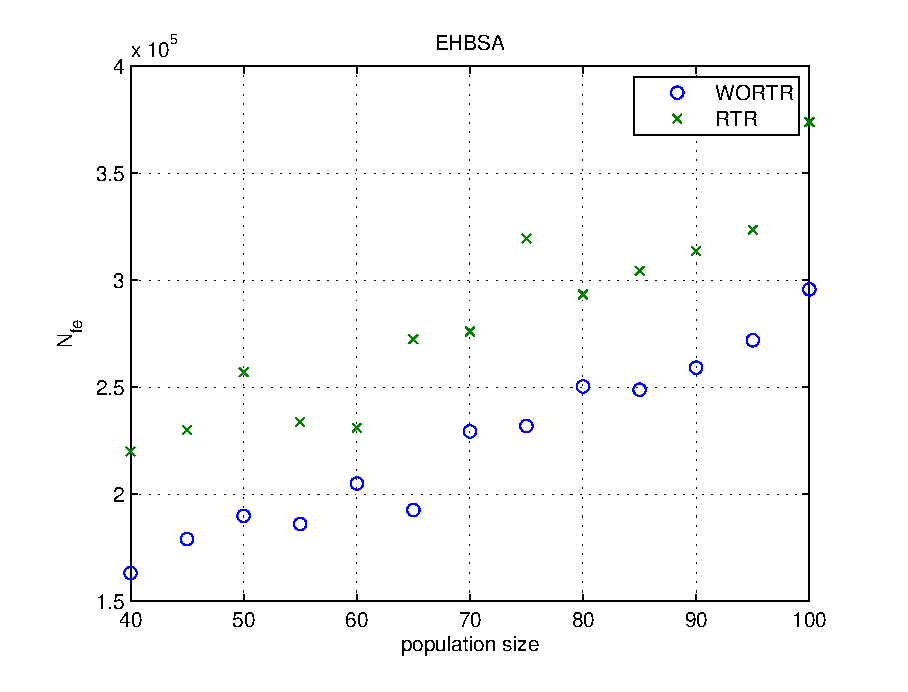
\includegraphics[width=\textwidth]{PN.eps}
            \caption{PopulationSize-$N_{fe}$}
        \end{subfigure}

        \caption{Results of runing EHBSA on benchmark eil51 20 times} 
        \label{fig:ehbsa_pf}
\end{figure}

In the figure \ref{fig:ehbsa_pf}, we respectively run EHBSA without RTR (EHBSAWORTR) and EHBSA with RTR (EHBSAWRTR) using edge distance with different population size 20 times on TSP.  Comparing the performance of EHBSAWORTR in the figure \ref{fig:ehbsa_pf}, we can see that $N_fe$ increases and failure decreases as population size growing up. The same conclusion holds when comparing the performance of EHBSAWRTR using edge distance. According to the above conclusion, we find that EHBSAWRTR with smaller population size outperforms EHBSAWORTR.

\subsection{Node Distance}
Node distance is calculated by each node at different position between two chromosomes. Let $D_{node} (i,j)$ denote the node distance between the two chromosomes $i$ and $j$. $D_{node} (i,j)$ is calculated as follows:\[D_{node} (i,j)=\sum_{k=0}^{ell-1} r_{i,j} (k), \]
where $r_{i,j} (k)$ is a function defined as \[r_{i,j} (k)=
\begin{cases}
1,  & \mbox{if }\pi_i(k)\neq \pi_j(k) \\
0, & \mbox{otherwise}
\end{cases}
.\]
In the above, $\pi_i(k)$  represents $k$-th gene of chromosome $i$.


\begin{figure}[htbp] 
        \centering
        \begin{subfigure}{0.45\textwidth}
            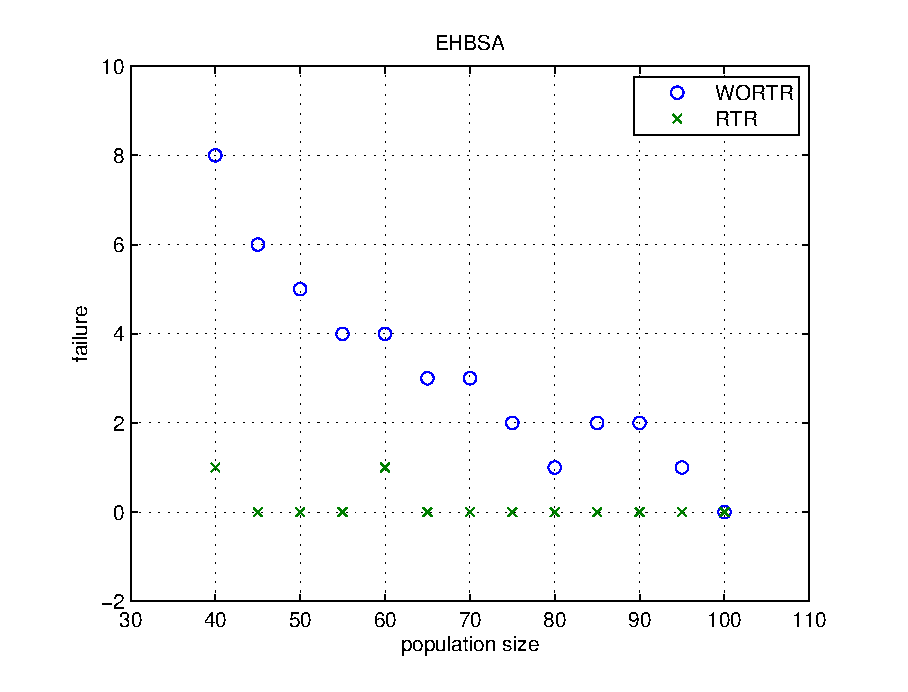
\includegraphics[width=\textwidth]{PF.eps}
            \caption{PopulationSize-Failure} 
        \end{subfigure}
        \begin{subfigure}{0.45\textwidth} 
            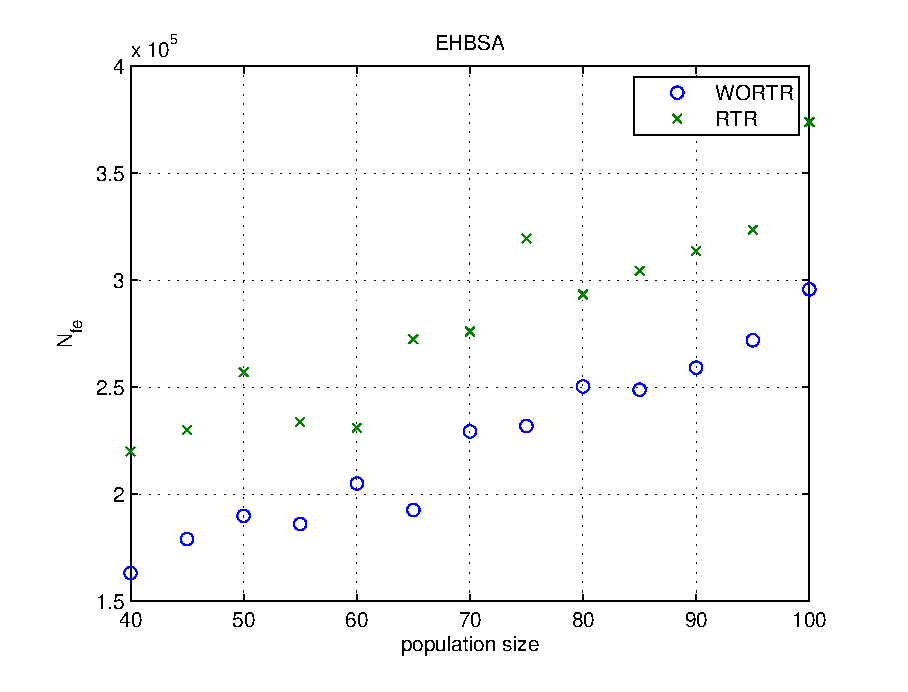
\includegraphics[width=\textwidth]{PN.eps}
            \caption{PopulationSize-$N_{fe}$}
        \end{subfigure}

        \caption{Results of runing NHBSA on benchmark ta031 20 times} 
        \label{fig:nhbsa_pf}
\end{figure}

In the figure \ref{fig:nhbsa_pf}, we respectively run NHBSA without RTR (NHBSAWORTR) and NHBSA with RTR (NHBSAWRTR) using node distance with different population size 20 times on FSSP.  The figure indicates that NHBSAWRTR with smaller population size outperforms NHBSAWORTR.


\subsection{Order Distance}
Order distance is calculated by different order of every pair of nodes between two chromosomes. Let $D_{order} (i,j)$ denote the order distance between the two chromosomes $i$ and $j$. $D_{order} (i,j)$ is calculated as follows:\[D_{order} (i,j)=\sum_u \sum_v \delta_{i,j}(u,v),\]
where $\delta_{i,j} (u,v)$ is a function defined as \[\delta_{i,j} (u,v)=
\begin{cases}
0,  & \mbox{if }\pi_i^{-1}(u)>\pi_i^{-1}(v)\mbox{ and } \pi_j^{-1}(u)>\pi_j^{-1}(v)  \\
1, & \mbox{otherwise.}
\end{cases}
\]
In the above, $\pi_i^{-1}(x)=y$ denotes that node $x$ represents the $y$-th gene of chromosome $i$.

\begin{figure}[htbp] 
        \centering
        \begin{subfigure}{0.45\textwidth}
            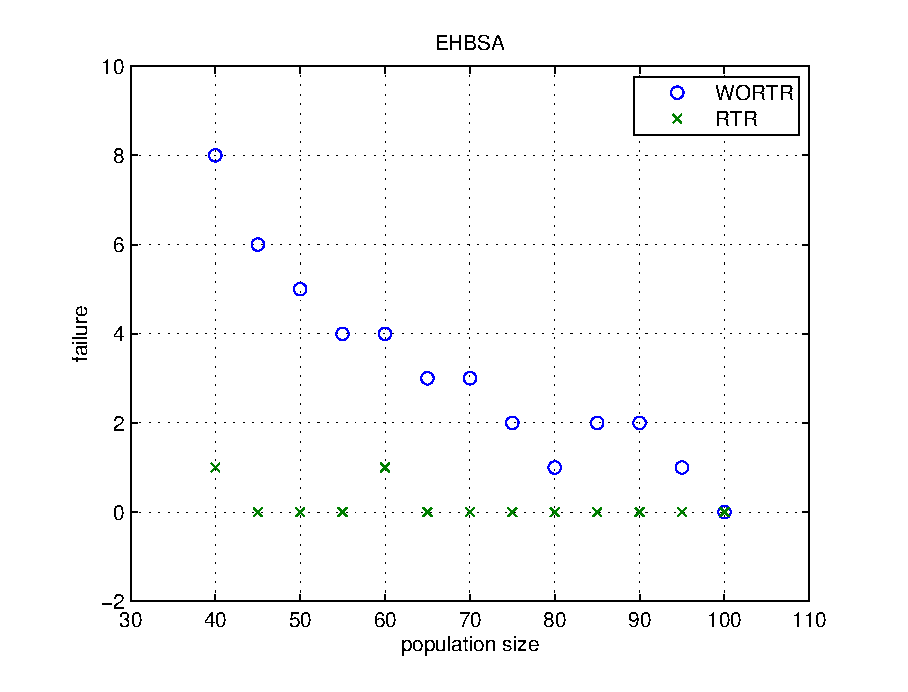
\includegraphics[width=\textwidth]{PF.eps}
            \caption{PopulationSize-Failure} 
        \end{subfigure}
        \begin{subfigure}{0.45\textwidth} 
            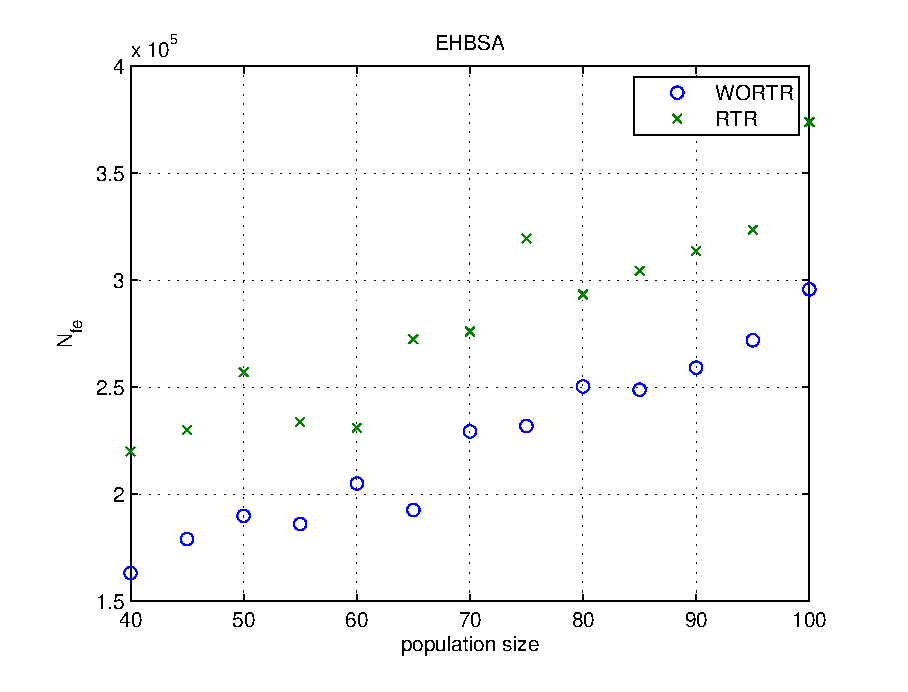
\includegraphics[width=\textwidth]{PN.eps}
            \caption{PopulationSize-$N_{fe}$}
        \end{subfigure}

        \caption{Results of runing Enum2(NHBSA,EHBSA) on benchmark t65i11xx 20 times} 
        \label{fig:enum2_pf}
\end{figure}

In the figure \ref{fig:enum2_pf}, we respectively run Enum2(NHBSA,EHBSA) without RTR (ENUM2WORTR) and Enum2(NHBSA,EHBSA) with RTR (ENUM2WRTR) using order distance with different population size 20 times on LOP.  The figure indicates that ENUM2WRTR with smaller population size outperforms ENUM2WORTR.


Now, we define three different types of distance functions for RTR on permutation problem . In the following section, we use these distance functions via different measure. 

\subsection{Weight Random Choice of Distance Measure}
Weight random choice of distance measure make a random choice with weighted probabilities. Let $D_{wrcdm} (i,j)$ denote the distance which calculated by weight random choice of distance measure between the two chromosomes $i$ and $j$. Assume that we only use edge distance and node distance, $D_{wrcdm} (i,j)$ is shown as follows:\[D_{wrcdm} (i,j)=
\begin{cases}
D_{edge} (i,j),  & \mbox{with probality } \frac{\alpha}{\alpha+\beta} \\
D_{node} (i,j), & \mbox{with probality } \frac{\beta}{\alpha+\beta} 
\end{cases}
,\]
where $\alpha$, $\beta$ and  ($0\leq$ $\alpha$, $\beta$ $\leq 1$ ) are constants. In this measure, we only choose distance once for one replacement. Besides, This measure can extend to more distance function.


\begin{figure}[htbp] 
        \centering
        \begin{subfigure}{0.45\textwidth}
            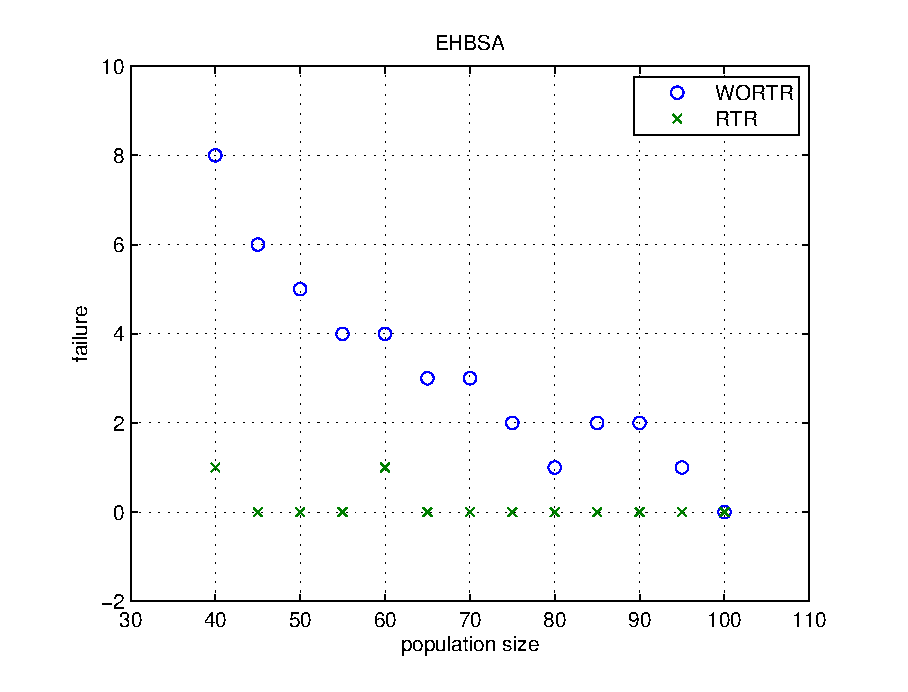
\includegraphics[width=\textwidth]{PF.eps}
            \caption{PopulationSize-Failure} 
        \end{subfigure}
        \begin{subfigure}{0.45\textwidth} 
            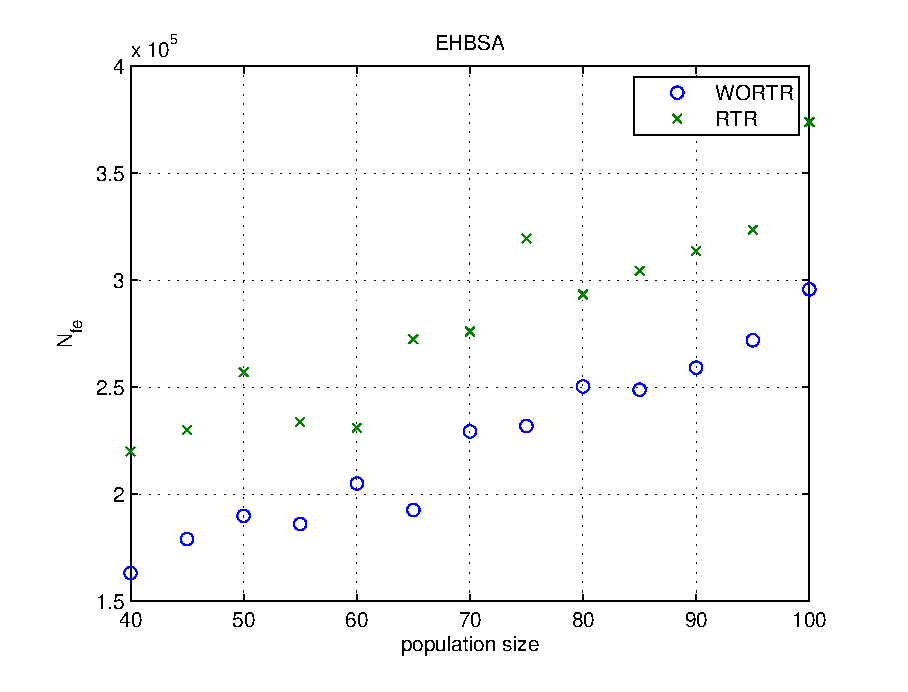
\includegraphics[width=\textwidth]{PN.eps}
            \caption{PopulationSize-$N_{fe}$}
        \end{subfigure}

        \caption{Results of runing Enum2(NHBSA,EHBSA) on benchmark t65i11xx 20 times} 
        \label{fig:enum2_sp}
\end{figure}

In the figure \ref{fig:enum2_sp}, we respectively run Enum2(NHBSA,EHBSA) with RTR (ENUM2WRTR) using weight random choice of distance measure with $\alpha$ which sweep in range [0,1] with different population size 20 times on LOP.  The figure indicates that weight random choice of distance measure outperforms  the measure which only use either edge distance or node distance.

 
\subsection{Weighted Summation Distance Measure}
Weighted summation distance measure determine distance by weighted summation of the three distance. Let $D_{wsdm} (i,j)$ denote the distance which calculated by weighted summation distance measure between the two chromosomes $i$ and $j$. For example, if we use edge distance, node distance and order distance. $D_{wsdm} (i,j)$ is shown as follows:\[D_{wsdm} (i,j)=\alpha D_{edge} (i,j)+\beta D_{node} (i,j)+\gamma D_{order} (i,j),\]
where $\alpha$, $\beta$ and $\gamma$ ($0\leq$ $\alpha$, $\beta$, $\gamma$ $\leq 1$) are constants.

\subsection{Model-associated Distance Measure}
Model-associated distance measure choose distance function according to model which chosen on model choosing phase. For example, enumeration method chosen EHBSA , so we use edge distance for RTR in this generation. Table \ref{tb:model_distance} show the relation between model and distance function.

\begin{table}[htbp]
    \centering
    \begin{tabular}{|l|l|}
    \hline
    \textbf{model}       & \textbf{distance}  \\ \hline
    \textbf{NHBSA} & node     	 \\ \hline
    \textbf{EHBSA} & edge   	\\ \hline
    \textbf{PLDEA} & order   	\\ \hline
  
    \end{tabular} 
    \caption{Corresponding distance function of model}
    \label{tb:model_distance}
\end{table}


\subsection{RTR Window Size}
\subsection{Empirical Study}